\documentclass[conference]{IEEEtran}

\usepackage{adjustbox}
\usepackage{amsmath}
\usepackage[nocompress]{cite}
\usepackage{float}
\usepackage{geometry}
\usepackage{graphicx}
\usepackage{listings}
\usepackage{pdflscape}
\usepackage{pgfgantt}
\usepgflibrary{patterns}
\usepackage{ragged2e}
\usepackage{url}
\usepackage{verbatim}

\newganttchartelement{contingency}{
    contingency/.style={
        shape=rectangle,
        inner sep=0pt,
        draw=black!50,
        very thick,
        pattern=north east lines
    }
}
\lstset{
    basicstyle=\small\ttfamily
}

\begin{document}
\newgeometry{vmargin=2.25cm, hmargin=2.25cm}
\title{Integrating CUDA into SNAP}


\author{\IEEEauthorblockN{Andrew Lamzed-Short}
\IEEEauthorblockA{ID: 1897268}}


\maketitle

%%%%%%%%%%%%%%%%%%%%%%%%%%%%%%%%%%%%%%%%%%

\begin{abstract}

Mini-applications (``miniapps'') are small-scale, representative versions of large-scale pieces of scientific- or engineering-focused software that seek to model the performance of an algorithm or program without the associated overhead of executing the larger program. This project seeks to examine the effects of altering the code base of one such miniapp called ``SNAP'' from utilising only traditional processing cores to incorporating a mixture of traditional computation and offloading applicable workloads to graphical processing cores with the aim to leverage their increased throughput and capabilities for single instruction, multiple data (SIMD) assignments. Ultimately the hope is to examine the performance of the resulting program to ascertain whether the modification is beneficial to the runtime of the algorithm, justifying if this change can be reflected in the larger-scale software SNAP represents.

To this end, this dissertation details a brief description to the field of High-Performance Computing (``HPC''), along with an introduction and description of the new field of miniapps. Overall aims of the project are outlined before related work in the field of miniapps, application modelling, and other HPC disciplines and projects are presented. This leads into an investigation into the existing SNAP code base and architecture, a thought out and concise approach to and overall design to a potential solution to the problem in hand, with the process finalised by a documented explanation as to the actual implementation. To conclude the report, a testing strategy and results are discussed and analysed, with concluding remarks as to the efficacy and efficiency of the project ending the report.

\end{abstract}

%%%%%%%%%%%%%%%%%%%%%%%%%%%%%%%%%%%%%%%%%%

\section{Introduction}
\label{sec:introduction}

\subsection{Background}

Modern, frontier-level science calls for large-scale, ambitious projects to answer some of the toughest questions. These projects often involve vast, complex simulations of natural phenomena, from modelling a human brain in one-to-one detail to answer questions about how memory works and how consciousness arises, to modelling the oceans to understand and make predictions about weather and climate change.

One of the predominant questions when designing these simulations is what architecture is best to run this program/suite of programs on. Different workloads and algorithms are designed for and benefit from certain types of computer architecture – some algorithms lend themselves well to being distributed over many cores, whereas others do not. Supercomputers of significant power are leveraged today for the foremost problems of our time: weather simulation and prediction\cite{metoffice}, human brain simulation\cite{humanbrain}, and simulated nuclear weapons testing\cite{nuclear}. The current state-of-the-art supercomputers, their power consumption and performance, are published in a list known as the ``Top500”\cite{top500}, with the most powerful supercomputer to date being ``Summit” housed at Oak Ridge National Laboratory, which can reach a performance of 143,500 Tflops/s\footnote{A ``flop” is an abbreviation for 1 floating-point, numerical operation, and a Tflop is a Teraflop, or $10\textsuperscript{12}$ floating point operations.} utilising 2,397,824 processing cores.

% [Supercomputer Architecture]
In general, supercomputers are comprised of numerous server racks housing many full computer systems – each one containing several CPUs, several graphics card, memory, and high-speed networking capabilities – all interconnected via a high-speed network to allow for communication and cooperation. The topology of the network connecting the computers can vary but two types tend to prevail: computer clusters, and grid computing. Clusters are composed of numerous components that are connected via a centralised resource management system to act as one individual system, with multiple clusters connected by a high-speed local area network (e.g. all in a single site) for low-latency communication; grid computing utilises clusters that are distributed geographically with the underlying assumption that a user of the system need not worry about where the computing resources they are going to be utilising are located – this provides reliability and access to and provision of additional resources on demand. The advantage of cluster computing for supercomputing over grid-based computing systems is stability and very low latency between nodes, as there isn’t a need for a high-speed internet connection between sites (also allowing the system to be air-gapped from the outside world for security purposes).

% [OpenMP and MPI – Software and programming paradigms to take advantage of this]
Since the era of Moore’s Law with respect to single-threaded/core workloads is coming to an end\cite{mooreslaw}, processors nowadays tend to have multiple cores, with consumer-grade electronics averaging four cores per chip, as can be seen in Figure \ref{fig:cpu_diagram} which details the architecture of a quad-core Intel Core i7 CPU. In addition to hyper-threading (2 threads per physical core), CPUs can have an effective/``logical” core count of twice that. Programming workloads to take advantage of this hardware-based parallelism can be challenging, and parallelising code over multiple nodes in a supercomputer can be even more so. This is where libraries such as OpenMP\footnote{\url{https://www.openmp.org/}} and MPI\footnote{\url{https://www.mpi-forum.org/}} come in. These are Application Programming Interfaces (APIs) that define how such a complex parallelisation system is to work, and each has multiple open-source implementations that allow for programmers to convert their code from single-threaded to multi-threaded over multiple clusters. It is these technologies predominantly that a large proportion of HPC applications are built with.

% \footnote{\url{https://m.hexus.net/tech/reviews/cpu/16187-intel-core-i7-x58-chipset-systems-go-fsb-invited}}
\begin{figure}
\centering
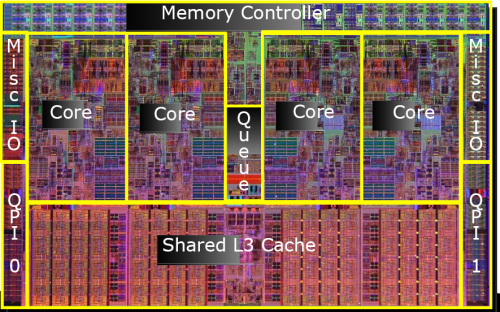
\includegraphics[width=0.45\textwidth]{images/cpu_diagram.png}
\caption{Quad-core Intel Core i7 CPU Architecture Diagram}
\label{fig:cpu_diagram}
\end{figure}

% [Use of GPUs – GPU Architecture]
Graphical Processing Units (GPU) are a newer technology than CPUs and serve a dedicated purpose of taking instructions from the CPU and performing multiple, hardware-based mathematical operations for translating three-dimensional shapes and coordinates into two-dimensional projections for rendering to a display, and runs multiple small programs called ``shaders” to handle colour and lighting. Due to the sheer amount of mathematical calculations that need to be performed to display something onto a display, GPUs have different architecture to that of a CPU. Modern graphics cards, such as Nvidia Turing architecture, pictured in Figure \ref{fig:gpu_diagram}, are composed of multiple stream processors, each divided into hundreds of small cores which perform a single integer or floating-point operation. This stream processing approach allows for vast parallel computation over a large dataset in a paradigm called ``single instruction multiple data” (SIMD).

% TODO: Develop this explanation further, how it works, etc.

This parallelism was previously reserved for image and video processing but a few years ago Nvidia released their CUDA API\cite{cuda_talk}\cite{CUDA} which allows developers to leverage the stream processing nature of the GPU for general-purpose computation. Scientific workloads from biomedical imaging\cite{luebke2008cuda} to deep learning\cite{tang2013deep} are now done on the GPU, and modern supercomputers, such as Summit, are built with large numbers of GPUs to accelerate workloads and perform previously-impossible simulations and workloads.

% \footnote{\url{https://devblogs.nvidia.com/nvidia-turing-architecture-in-depth/}}
\begin{figure}
\centering
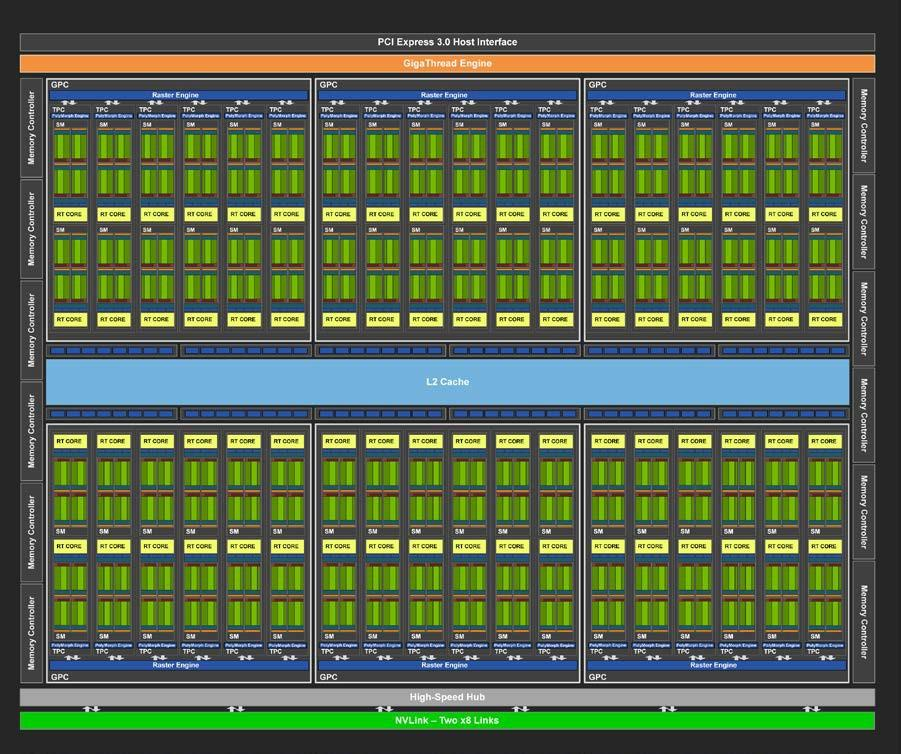
\includegraphics[width=0.45\textwidth]{images/gpu_diagram.jpg}
\caption{Nvidia Turing GPU Streaming Multiprocessor Architecture Diagram}
\label{fig:gpu_diagram}
\end{figure}

% Miniapps
Mini-applications (``mini-app”) are a new area within the field of High Performance Computing (HPC). These applications are small, self-contained proxies for real applications (typically relating to simulation of physical phenomena) to quickly and concisely explore a parameter space, leading to focused and interesting performance results to investigate potential scaling and run-time issues or trade-offs\cite{miniapps}. Mini-apps capture the behaviour and essence of their parent applications primarily because of two characteristics of many applications running on distributed systems: the performance of an application will mainly be constituted by the performance of a small subset of the code, and many of the physical models that constitute the rest of the application are mathematically distinct and generally have similar performance characteristics\cite{miniapps}.

\subsection{Objectives}

The SN (Discrete Ordinates) Application Proxy (SNAP) is a mini-app that acts as a proxy for discrete ordinates particle transport. It is modelled off another production simulation program developed by the Los Alamos National Laboratory (``LANL'') called PARTISN, which solves the linear Boltzmann transport equation (TE)\footnote{Boltzmann Equation: \url{https://en.wikipedia.org/wiki/Boltzmann_equation}\raggedright}, simulating neutron criticality and time-independent neutron leakage problems\cite{partisn} in a multi-dimensional phase space. SNAP is a proxy to PARTISN because it provides a concise solution to a discretised, approximated version (though with no real-world relevance) of the same problem PARTISN solves, providing the same data layout, the same number of operations, and loads elements into arrays in approximately the same order.

The SNAP algorithm works by defining the phase space as seven dimensions: three in space (x, y, z), two in angle (octants, angles), one in energy (groups, or energy-based bins of particles), and one of time (time step). SNAP sweeps across the spatial mesh, starting in each of the octants proceeding towards the antipodal octant, performing a time-dependent calculation in each cell using information from the previous time-step and surrounding cells. This motion forms a wave-front motion that sweeps across the three-dimensional space from corner to corner, with work being divided along each diagonal for parallel execution

With this mini-app in mind, we define three key objectives that the project shall solve. Taken together, these will provide a holistic overview as to the validity and efficacy of this approach of converting CPU-bound parallelised algorithms to utilise the GPU instead (where appropriate). With the SNAP algorithm and open-source repository (specifically the C-based port of the code) in mind, the three objectives are:

\begin{itemize}

\item To instrument, profile, and analyse the current implementation of the code in order to identify areas of the code in which it would be applicable and beneficial to convert to CUDA-based parallelisation.

\item Using the identified areas found in problem 1, to fork the current C-based port of the SNAP GitHub repository\footnote{\url{https://github.com/lanl/SNAP}} and convert the candidate components and routines from OpenMP to utilise the CUDA libraries instead.

\item Following the reimplementation of the algorithm to CUDA technology, the last step is to analyse and evaluate the efficiency and efficacy of the new solution in comparison to the previous CPU-based approach. Ideally, a theoretical maximum efficiency of the approach will also be calculated mathematically, and the actual implementation compared against this as another measure of success.

\end{itemize}

%%%%%%%%%%%%%%%%%%%%%%%%%%%%%%%%%%%%%%%%%%

\subsection{Related Work}

A seminal work in the field of mini-apps was written by Heroux et al\cite{miniapps}, defining the paradigm. Their Mantevo mini-app suite has show successful development of mini-apps, such as MiniFE for finite element analysis and MiniMD for molecular dynamics simulations, to demonstrate their versatility and applicability. Others have demonstrated such success in other areas, such as Mallinson et al with ``CloverLeaf”\cite{mallinson2013cloverleaf}, and Los Alamos National Lab (\url{https://www.lanl.gov/projects/codesign/proxy-apps/lanl/index.php}). Mini-apps have been shown to produce similar performance characteristics to their fully-fledged counterparts\cite{miniapps}, adding to the efficacy of the paradigm.

General-purpose simulations on GPUs have been studied for a long time, with GPUs being a core part of modern computing clusters\cite{debardeleben2013gpu}. Strong-scaling across multiple GPUs\cite{glaser2015strong} is the ideal approach. Consideration is taken also for conversion of existing code bases\cite{zhou2011gpu} and new, bespoke solutions designed with GPU architecture utilisation in mind\cite{glaser2015strong}. Bespoke solutions offer superior code architecture and speed, meaning calculation of theoretical maximum performance increase for a pre-existing code base will have to take this into account.

Writing GPU targeted mini-apps in a developing area of work. Baker et al\cite{baker2012high} discuss implementation details of converting the KBA sweep algorithm of the Denovo code system to run on Nvidia Titan GPU. Mallinson et al\cite{mallinson2013cloverleaf} demonstrate too with CloverLeaf the performance advantages GPU-based architecture targeting can have over purely CPU-based versions. It is important to note that these performance increases might not necessarily be completely reflected in SNAP’s algorithm due to other considerations, such as the scaling characteristics of the algorithm\cite{shoukourian2014predicting} and communication technologies as highlighted by Glaser et al\cite{glaser2015strong}.

Performance of mini-apps with respect to CPU- and GPU-based parallelisation frameworks have been explored previously and show promising results which add credence to the motivation of this project. Notably Martineau et al\cite{martineau2017productivity} reached the conclusion that compiling mini-apps to CUDA resulted in greater efficiencies compared to other targets, though care is needed to consider the implementation (especially with respect to data accesses) to avoid the compiler introducing performance penalties.

Development of the solution must still mimic the behaviour of the original application however, so care must be taken to preserve this. Heroux et al\cite{miniapps} and Messer et al\cite{messer2015developing} outline the fundamental principles that a mini-app must adhere to and the considerations of forming a mini-app from the base application – all of which would help form testing criteria for this project and future projects to help preserve results and intrinsic behaviour.

%%%%%%%%%%%%%%%%%%%%%%%%%%%%%%%%%%%%%%%%%%

\section{Project Management}
\label{sec:projectmgmt}

Several factors need to be considered when developing a software project. Management of time constraints is discussed first as producing a novel software project as part of an entire Masters course will run into difficulty - mostly with conflicting or overlapping deadlines but also due to the inevitable problems associated with any software development project. Following on from this, it is also key to highlight how the code was managed and versioned so as to preserve the history of changes and the progression of the project, should ideas need to be experimented with or code recovered should anything unforeseen occur.

\subsection{Time Constraints}

Time constraints are always a pressing and important factor to consider when starting a large project. The external largest constraints imposed on this project would be the time required to complete several overlapping coursework assignments for various MSc modules, in addition to setting aside time to adequately prepare for and take the end of year exams in June and July. To manage these obstacles, the timeline presented in Figure \ref{fig:gantt_chart} was developed early on in the research phase of the project to delineate when and how long certain key stages of development were to last for, with the potential speed-bumps to this project's progression (i.e. MSc examinations) highlighted and accounted for.

\begin{figure*}[ht]
    \centering
    \ganttset{calendar week text=\small{\startday}}
    \begin{ganttchart}[
        y unit chart=0.75cm,
        hgrid,x unit=0.1cm,
        hgrid style/.style={draw=black!5, line width=.75pt},
        milestone/.style={fill=black, draw=white, rounded corners=4pt},
        milestone label font={\it\scriptsize},
        bar label node/.style={text width=2cm,align=right,font=\scriptsize\RaggedLeft,anchor=east},
        group label node/.style={text width=2cm,align=right,font=\bf\scriptsize\RaggedLeft,anchor=east},
        title label anchor/.style={below=-1.6ex},
        time slot format=little-endian]{01-05-2019}{26-09-2019}
    \gantttitlecalendar{month=shortname, week=4} \\
    \ganttgroup{Project Duration}{01-05-2019}{26-09-19}\\
    % Impediments
    \ganttmilestone{Examinations}{13-05-19}
    \ganttmilestone[inline=false]{}{30-05-19}
    \ganttmilestone[inline=false]{}{31-05-19}
    \ganttmilestone[inline=false]{}{01-06-19}
    \ganttmilestone[inline=false]{}{05-06-19}
    \ganttmilestone[inline=false]{}{08-06-19}\\
    % Investigation
    \ganttgroup{Investigation}{01-05-19}{24-06-19}
    \ganttcontingency[]{}{25-06-19}{02-07-19}\\
    \ganttbar{Preliminary Exploration}{01-05-19}{01-06-19}\\
    \ganttbar{Codebase Examination}{03-05-19}{17-06-19}\\
    \ganttbar{Learning CUDA}{10-06-19}{24-06-19}\\
    % Design
    \ganttgroup{Design}{05-06-19}{31-07-19}
    \ganttcontingency[]{}{01-08-19}{08-08-19}\\
    \ganttbar{Mathematical Model}{05-06-19}{15-07-19} \\
    \ganttbar{Test Harness Concept}{01-07-19}{15-07-19}\\
    \ganttbar{Ideation}{01-07-19}{31-07-19}\\
    % Design and implementation
    \ganttgroup{Implementation}{01-07-19}{18-08-19}
    \ganttcontingency[]{}{19-08-19}{30-08-19}\\
    % Testing
    \ganttgroup{Testing}{15-07-19}{30-08-19}
    \ganttcontingency[]{}{31-08-19}{07-09-19}\\
    \ganttbar{Local Profiling and Benchmarking}{15-07-19}{19-08-19} \\
    \ganttbar{Cluster Profiling and Benchmarking}{29-07-19}{30-08-19} \\
    % Dissertation
    \ganttgroup{Dissertation}{12-08-19}{26-09-19} \\
    \ganttbar{Writing}{12-08-19}{26-09-19} \\
    \ganttbar{Proof Reading and Editing}{5-09-19}{26-09-19}
    \end{ganttchart}
    
    \caption{The Proposed Timeline of this Project}
    \label{fig:gantt_chart}
\end{figure*}

During an early presentation and review of the project, it was made clear that no contingency had been built into the timeline of the project that would alleviate pressure in the event of unfortunate circumstances arriving - whether that be unavailability of resources, issues arising during testing, having to adjust the design, or the typical software development issue of features taking longer to develop than initially estimated. Hence, in Figure \ref{fig:gantt_chart}, contingency periods for overall stages of the project are blocked out in the striped areas shown to allow the project to stay on course and on-time.

\subsection{Source Control}

Every major modern software development project uses source control at its core. Source control is key to backing up software in an external repository, maintaining multiple versions of the same code base in a linear or parallelised fashion to be able to restore the code to a former state or maintain a legacy version alongside a more modern version (for instance), and for branching code to allow many developers to work on potentially overlapping areas of the code at once.

To this end, a decision was made to version control the code for the project using \texttt{git}. Other source control alternatives were considered but \texttt{git} has all of the features discussed in addition to being widely supported, an industry standard, and repository hosting services GitHub and GitLab being two of the most popular offerings available. GitHub offers free hosting for public repositories and is already where the original SNAP repository is hosted.

With this in mind, LANL's SNAP repository was forked into a new repository located at \url{https://www.github.com/alshort/snap}. From here it will be cloned onto the local development machine and worked upon in a linear fashion, branching code were experimental code is to be created. Tags will be used to denote stable versions when they are created.

In terms of the specific source control methodology used, the project will be managed using an industry standard git branching model called ``git-flow''\cite{gitflow}. The model is illustrated in Figure \ref{fig:gitflow}.

\begin{figure}[!h]
    \centering
    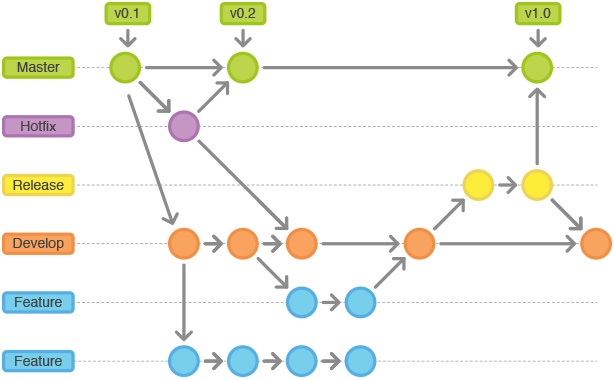
\includegraphics[width=0.4\textwidth]{images/gitflow.png}
    \caption{Visual map of the git flow methodology}
    \label{fig:gitflow}
\end{figure}

The methodology specifically involves a master branch maintained with only tagged releases, and a develop branch that all of the development is done on. Features and hotfixes are done on separate branches and merged back into their parent branch, with testing and release-candidate branches spawned off a fixed point on the develop branch. After complete testing and verification that everything works, they will get merged down into the master branch and a new version tagged.

\subsection{Hardware and Software}

Intel's port of SNAP relies on very particular tooling and platform decisions so most of the decisions with regards to testing and development tooling were already determined ahead of time. Furthermore, the decision to utilise CUDA as a platform to accelerate the performance of the mini-app also additional hardware requirements in an Nvidia-based GPU and accompanying drivers and development suites. If the modifications to the code base are successful, it is hoped to execute the software under both a local testing environment and a cluster computing environment at the University of Warwick's Department of Computer Science. Details of both of the set-ups follow.

\subsubsection{Local Development Platform}
\label{subsubsec:projmgmt_localtesting}

It is sufficient enough to be able to compile, execute, and test both the stock SNAP application as well as a GPU-accelerated alteration on a typical home desktop computer as of time of writing, given some particular brand-alignments/proprietary technologies are in mind when the machine is purchased or built. As such, hardware specifications of the home desktop computer used as the local development environment are as follows:

\begin{itemize}
    \item \textbf{Intel® Core™ i7-6700K CPU}: A single quad-core, consumer-grade, overclockable CPU produced by Intel as part of their 6th generation ``Skylake'' line of processors. It has a clock speed of 4GHz (overclockable) and comes as standard with hyper-threading enabled for an (apparent) core count of 8.
    \item \textbf{Nvidia GeForce GTX 1070 graphics card}: Pascal architecture-based GPU that supports the CUDA Compute functionality. In terms of hardware specifications, it has a 1.5GHz base/core clock speed, 8GB of GDDR5 memory, and 15 streaming multi-processors for parallelism.
    \item \textbf{16GB DDR4 RAM}.
    \item \textbf{Samsung 860 EVO SSD}: Storage disk for the Ubuntu operating system the project with be developed and tested on - both the original SNAP porters and cluster environment use the platform and tools on it, so the choice was made mainly for feature-parity and consistency (see below).
\end{itemize}

This set-up allows for the compilation and testing of the current implementation of SNAP as well as a CUDA-accelerated version by both having the correct hardware that the software is and will be built for, while also being flexible enough in order to test the programs under a range of different inputs and constraints (such as having anywhere from 1 to 8 threads to run the program on). Whilst newer generation Intel processors would be even more ideal, such as the Intel® Core™ i9-7960X 16-core processor, the current hardware more than suffices enough to yield a satisfactory picture of the performance characteristics of the MPI and OpenMP implementation and limitations for this application.

\subsubsection{Computing Clusters}
\label{subsubsec:clusters}

% Compute nodes: Lenovo NeXtScale nx360 M5 servers with 2 x Intel Xeon E5-2630 v3 2.4 GHz (Haswell) 8-core processors; 16 cores per node; 203 nodes; 3488 cores; 64 GB DDR4 memory per node / 4 GB per core
% GPU nodes: 8 x NVIDIA Tesla K80 GPU cards; 2 GPU cards per node; 4 GPUs per node; 4 nodes; 64 GB DDR4 memory per node
% Phi nodes: 8 x Xeon Phi 7120P; 2 Phi processors per node; 4 nodes; 64 GB DDR4 memory per node
% Fat nodes: 128 x Intel Xeon E7-4809 v3 2.0 GHz Haswell cores; 32 cores per node; 4 nodes; 1 TB DDR3 memory per node; 1 x NVIDIA GRID K2 GPU per node
% Interconnect: QLogic TrueScale InfiniBand
% Storage: 0.5 PB GPFS
% OS: CentOS 6.x
% Workload Manager: Slurm
% Commissioned: Oct 2015
% Expected EOL: Oct 2019
% Intended use: Parallel computing

There are two local high-performance computing clusters available for use at the University of Warwick that are ideal to test the potential multi-GPU capabilities of the end solution. Tinis and Orac are both similar in capabilities but differ in terms of architecture and hardware - Orac being comprised of newer hardware whilst Tinis is expected to reach end-of-life in October 2019\cite{warwickclusters}.

Tinis will be the focus of the cluster-based testing of the GPU-accelerated program because of more than capable hardware to prove or disprove the effectiveness of the final solution, in addition to additional familiarity with it due to the teachings of the CS402 course that is part of the MSc Computer Science program. There are many different types of nodes built into the cluster for handling a wide range of applications: compute nodes, GPU nodes, Phi nodes, and Fat nodes. The Phi and Compute nodes are purely computationally focused, so are not appropriate for the needs of this application. GPU nodes will only have the essential hardware in order to operate several graphics devices per node, which again is not appropriate, as this application will need a mixture of CPU and GPU power. Fat nodes have both high-power server processors and Nvidia graphics cards in each node, making them ideal. The specifications for them, as well as the crucial components of the system as a whole, are as follows:

\begin{itemize}
    \item 4 nodes, each composed of:
    \begin{itemize}
        \item 32 x Intel Xeon E7-4809 v3 2.0 GHz Haswell cores
        \item 1TB DDR3 memory
        \item 1 x NVIDIA GRID K2 GPU per node (CUDA capable)
    \end{itemize}
    \item Networking provided by QLogic TrueScale InfiniBand which supports many-gigabit per second transfer speeds between nodes.
    \item CentOS 6.x as the underlying operating system. It's a robust, reliable distribution of Linux that incorporates all of the hardware in the cluster under one management system.
    \item Slurm as the workload manager for submitting the program as a job to any of the available nodes.
\end{itemize}

In total, this provides, in the best-case scenario, a total of 128 traditional processing cores and 4 high-end graphical processing devices (each with two GK104 GPUs\footnote{As per the specification of the device: \url{https://www.nvidia.com/content/grid/pdf/GRID_K2_BD-06580-001_v02.pdf}}). A hybrid program that has multi-CPU and multi-GPU capabilities should be able to leverage a significant portion of the power provided should the threading and data orchestration work.

Having multiple cores for both types of devices will allow for testing over a range of different configurations of traditional-only computation, and a varying amount of hybrid resources to find the optimal amount as well as any bottlenecks or trends in performance that might appear.

\subsubsection{Software}

Working with an existing and established code base means adhering to existing tool chains where possible in order to correctly compile the software and to have an identical executing environment to run the program in to ensure the program behaves as intended. Thus, most software choices were predetermined for the project. Where nothing was chosen already, the rest of the choices were made due to personal preference, familiarity, or significant advantages were present that made them ideal for their role. All the options are listed below:

\begin{itemize}
    \item \textbf{Ubuntu}: An open-source flavour of Linux favoured by developers for its rich tooling, reliance on shells and terminals and the power they provide, and ability to work at multiple levels (high or low depending upon the circumstances).
    \item \textbf{bash}: A ``shell'' that provides a command-line interface to execute programs and interact with a Linux-based operating system. Useful for simplicity and for automation purposes with shell scripts, calling make files to handle compilation etc.
    \item \textbf{Visual Studio Code}: A cross-platform, automatable text editor with multiple extensions available. Used specifically in this project for its syntax highlighting capabilities for C, C++, Make, Bash, and \LaTeX, as well as executable tasks to automate routines with its built-in terminal, and the latex-workshop extension for dynamically building, parsing, and previewing \LaTeX documents. The tasks developed for this project can be found in the \texttt{.vscode/tasks.json} file located in the source code.
    \item \textbf{mpiicc}: Proprietary compiler for compiling code that uses both the MPI parallelisation specifications and Intel-specific C- and C++-based code.
    \item \textbf{make}: Shell-based program that follows a given set of recipes within a Makefile for compiling multiple dependent parts of source code. Intel provided one to build their SNAP port with their \texttt{mpiicc} compiler, and this will further be modified later to incorporate other files and tools.
    \item \textbf{nvcc}: Proprietary compiler produced by Nvidia to compile C++ code that targets the CUDA Compute capabilities of their compatible graphics cards.
    \item \textbf{pdflatex, bibtex}: Back-end programs for Visual Studio Code and latex-workshop to use to built \LaTeX and accompanying bibliography files. Errors and output are parsed and displayed in Visual Studio Code's in-built terminal for an enhanced and compact workflow.
\end{itemize}

Any additional programs used are merely an intrinsic feature of the operating system used. Features like \texttt{ssh} to remote into the Tinis computing cluster, \texttt{git} for fine-tuned version control, and other utilities are found on most development systems.


%%%%%%%%%%%%%%%%%%%%%%%%%%%%%%%%%%%%%%%%%%

\section{Investigation}
\label{sec:investigation}

All code previously and actively developed by a third-party is legacy code. SNAP, with its various ports, is no different. The original foundation is developed in FORTRAN90 as this language is still used in many areas of HPC 

\subsection{SNAP Repository Cloning and Documentation Review}

Initial plans involved gaining a fundamental understanding of the nature of the algorithms and data structures that the SNAP program utilises in order to effectively emulate and model its larger counterpart program. LANL provide the full FORTRAN90 source code, in addition to several ports into other, different languages, in the GitHub repository located at \url{https://www.github.com/lanl/snap/}. For the purposes of this project, it will be Intel's C-based port that shall be modified and examined due to ease of use for compilation and finding the appropriate tooling (compilers, syntax highlighters etc.) as well as increased familiarity with the language over FORTRAN90.

The entire repository was forked on GitHub for the purposes of modification. It can be found at \url{https://www.github.com/alshort/snap}. All non-C-based ports were removed from the repository in addition to any miscellaneous files and documentation as these were superfluous. Only the \texttt{qasnap/} and the \texttt{src/} directories (of Intel's code) were kept as these would be the only necessary sets of code needed to build, execute, and test SNAP and this project's proposed modifications.

In the main repository, various presentations and documentation are provided that discuss the reasoning behind creating SNAP, background behind PARTISN and the code SNAP was seeking to model, as well as an overview of some of the implementation details of the main constituent of the approach LANL and Intel took: the ``sweep'' algorithm.

\subsection{Execution, Profiling, and Investigation of Code}

\subsubsection{Compilation}
\label{subsubsec:inv_compilation}

Intel chose to target the C-based port of SNAP towards Intel-based CPUs, hence the decision, as outlined in section \ref{sec:projectmgmt}, to use a machine to locally test the program having an Intel Core i7-6700K CPU. This decision was made due to the original port writers' knowledge of the benefits that the architecture and proprietary improvements could bring to a strictly MPI-based implementation of SNAP. One such proprietary optimisation is the \texttt{-xAVX} compiler flag that was introduced from the ``Sandy Bridge''-line of Intel CPUs onwards that introduced the option to include new instructions (and expanded old instructions) that allowed for operations - specifically fused multiply-accumulate (FMA) operations - for the execution of some SIMD workloads on floating-point data\cite{KanterIntel}. This operation is similar in principle and execution to the SIMD nature of data manipulation on a standard GPU but cannot compare to the speed or scale of that which is obtainable on streaming multi-processors.

GNU make is used to compile all facets of the program, with the main compiler being \texttt{mpiicc}. Whilst \texttt{gcc} is typically used to compile regular, standard C and C++ code, \texttt{icc} is Intel's C++ compiler that was built in order to specifically optimise code to run on Intel-created architectures. This includes optimisations for how memory is specifically accessed, how thread-based parallelisation is handled with regards to the OpenMP specification, data layout improvements, and support for modern iterations of C++ language specifications\footnote{\url{https://software.intel.com/en-us/c-compilers}}. \texttt{mpiicc} is an HPC-specific version of the \texttt{icc} compiler that utilises message-passing library built for use with the \texttt{icc} program (in particular its C-based capabilities). This library implements the Message Passing Interface (MPI) specification version 3.1\cite{intel-mpi-ref} to allow for bi-directional inter-process communication, regardless of how those processes are mapped to the underlying hardware.

Whilst provided in an operational state, this provision is predicated on the correct resources and dependencies being installed and linked up on the host system. Installation of Intel's MPI libraries is straight-forward but ensuring that they will operate correctly when called can be an issue.

One of the foremost scripts devised when the project started was a bash script that ran several commands in order to register locations and associations of binary files that are a core part of Intel's MPI libraries with the host shell (standard bash in this instance) so that the environment could call upon these when needed by either the compiler or the runtime code. Figure \ref{fig:source_list} shows this script of ``source'' commands. The execution of this script was appended to the environment's \texttt{.bashrc} file in order for it to get executed before each bash shell has finished initialisation, allowing for the references to be available all to time to accelerate testing and development.

\begin{figure}[h]
    \centering
    \begin{lstlisting}[language=bash, breaklines]
#!/bin/sh
. ~/intel/bin/compilervars.sh -arch intel64 -platform linux
. ~/intel/mkl/bin/mklvars.sh intel64
. ~/intel/bin/iccvars.sh -arch intel64 -platform linux
. ~/intel/compilers_and_libraries/linux/mpi/intel64/bin/mpivars.sh 
    \end{lstlisting}
    \caption{intel.sh}
    \label{fig:source_list}
\end{figure}


\subsubsection{Understanding the Input Data}

Provided as part of the original SNAP repository is a folder called \texttt{qasnap}. In this folder resides several input and respective output files for quality assurance and testing. Executing the binary file as above and then comparing it line-by-line to the model output will highlight any discrepancies in the accuracy of the answer - any incorrect modification to the algorithm will flag as an inaccuracy. (The output files also output the timings of the execution but this will be guaranteed to be different on any machine.)

The input data is in a proprietary format in a whitespace-indented file. Due to the fact that the code is a proprietary piece of software developed for a specific task, it is understandable that the documentation is sparse in places, especially with regards to the meaning of these key-value pairs in context.

LANL is in the United States of America, so direct support requests would be costly in terms of time and constrained by time zones, in addition to being potentially low-priority items. Mercifully, within Intel's C-based port contains useful commenting. Hence, alongside analysis and reading of the code, use and meaning of the input variables can be inferred from context for the most part. Figure \ref{table:input-data} shows several of the more essential items. 

\begin{figure}[h]
    \centering
    \begin{tabular}{| p{1.7cm} | p{5.7cm} |}
        \hline
        Variable & Use \\
        \hline
        \texttt{nthreads} & Number of threads per process. \\
        \texttt{npey} & Number of parallel processing inputs in the y direction. \\
        \texttt{npez} & Number of parallel processing inputs in the z direction. \\
        \texttt{ndimen} & Total number of dimensions to the grid. \\
        \hline
    \end{tabular}
    \caption{Important variables defined in the input data}
    \label{table:input-data}
\end{figure}

\dots

\subsubsection{Execution}
% different threads, input data, averaging

Following successful compilation of the SNAP executable, several executions were performed under various environmental-constraints and input data to ascertain the current limitations and performance of the code base as it stands.

Due to its reliance on MPI for its processing, the compiled program is executed via Intel's \texttt{mpirun} program at the command line with an argument specifying the size of the MPI communication channel (or overall number of parallelised processes), the \texttt{-np} command-line argument, to divide the work into, as opposed to calling the executable by itself. An example execution is as follows:

\begin{lstlisting}[breaklines]
mpirun -np 4 src/snap_mkl_vml --fi qasnap/center_src/in01 --fo test.out
\end{lstlisting}

Figure \ref{fig:snap-successful-run} demonstrates the output of a successful execution of a given input.

\begin{figure}[!h]
    \centering
    \begin{lstlisting}[breaklines]
andy@pc:~/uni/snap/src$ mpirun -np 4 ./snap_cpu --fi ../qasnap/center_src/in01 --fo test.out

*WARNING: PINIT_OMP: NTHREADS>MAX_THREADS; reset to MAX_THREADS
Success! Done in a SNAP!
    \end{lstlisting}
    \caption{A successful execution of the compiled snap\_mkl\_vml binary}
    \label{fig:snap-successful-run}
\end{figure}

It was identified early on into the testing - whilst undocumented, it could be said to be a core feature of the MPI specification itself - that defining an \texttt{-np} value that is not a whole multiple of the product of the defined grid geometry from the input data (\texttt{npey} $ \times $ \texttt{npez}) then the runtime configuration cannot work out how to divide up the workload into whole, viable chunks to send to all processes. Figure \ref{fig:snap-unsuccessful-run} shows the error message provided in this scenario.

\begin{figure}[h]
    \centering
    \begin{lstlisting}[breaklines]
andy@pc:~/uni/snap/src$ mpirun -np 1 ./snap_cpu --fi ../qasnap/center_src/in01 --fo test.out
Abort(202454796) on node 0 (rank 0 in comm 0): Fatal error in PMPI_Cart_create: Invalid argument, error stack:
PMPI_Cart_create(325).....: MPI_Cart_create(comm=0x84000002, ndims=2, dims=0x7ffd07f649b0, periods=0x7ffd07f649b8, reorder=1, comm_cart=0x7ffd07f64bac) failed
MPIR_Cart_create_impl(194): 
MPIR_Cart_create(58)......: Size of the communicator (1) is smaller than the size of the Cartesian topology (4)
    \end{lstlisting}
    \caption{An unsuccessful execution of the snap\_mkl\_vml binary due to imposed multi-processing limitations}
    \label{fig:snap-unsuccessful-run}
\end{figure}

Ascertaining the characteristics, properties, and limitations of an existing code base before modification provides vital insight that can guide the rest of development. Using the limitation in terms of number of processes to run a sample execution on will guide the test plan in particular ()


\subsection{\texttt{gprof}}
% Print out of "example" analysis

The central issue of profiling parallelised code is that of ascertaining which functions calls are being called and calculating the total amount of time spent there (amongst obtaining other metrics and measurements of interest). In serial code, this task is easy. However, parallel code can be distributed over multiple nodes, processors, and/or threads depending on the resources available, the way the program works, and how the scheduling system decides to allocate work and timeslots. All of this must be orchestrated together, tracked, and aggregated to form one cohesive picture of what the application did on the execution of interest.

\texttt{gprof} is a command-line based profiling tool that displays the call graph profile data of any C, Pascal, or Fortran code it was set to monitor\footnote{On the provision that the code in question was compiled with the \texttt{-pg} parameter beforehand.}. When the compiled binary is run, it will produce a single \texttt{gmon.out} file containing the pertinent profile data. This data is consumed by the main gprof application for analysis. In terms of the output it can produce, \texttt{gprof} is able to relate the \texttt{gmon.out} profile data to the program's symbol table to output a call graph of functions and the functions that call them and how they related to one another. In addition to this, \texttt{gprof} can also output the total number of calls of a function and how long the program spend inside each subroutine.

In order to cater for parallel programs, \texttt{gprof} is able to sum the results of multiple profile data files into one for a general overview. Producing the multiple traces is performed by setting the \texttt{GMON\_OUT\_PREFIX} environment variable to differentiate the traces. Setting this variable to ``\texttt{gmon.out-}'' will cause \texttt{gprof} to append the process's ID to the end of the prefix, producing several files pertaining to the run of the program - one for each process. \texttt{gprof -s} will sum these together and produce a useful, informative result.

Performing this profiling on the standard SNAP application compiled earlier in the investigation yield the table shown in Figure \ref{table:gprof_log}. In the table is a truncated subset of the five most called and time-intensive subroutines. Multiple executions of the program exhibit near identical characteristics in terms of the subroutines reported back by the \texttt{gprof} tool.

\begin{figure}[!h]
    \centering
    \begin{tabular}{ | c | c | c | c | }
\hline
\% Time & Cumulative Secs & Calls & Name \\
\hline
66.67 & 0.02 & 14976 & \texttt{dim3\_sweep} \\
33.33 & 0.02 & 14976 & \texttt{sweep} \\
0.00  & 0.03 & 29952 & \texttt{precv\_d\_3d} \\
0.00  & 0.03 & 29952 & \texttt{psend\_d\_3d} \\
0.00  & 0.03 & 14976 & \texttt{octsweep} \\
\hline
    \end{tabular}
    \caption{Amalgamated \texttt{gprof} log (truncated to top 5 rows)}
    \label{table:gprof_log}
\end{figure}

Two of the functions are associated with intrinsic data transmission across MPI processes. The others are part of the main transport sweep algorithm that is a central tenant of the SNAP program. This was to be expected but is now experimentally confirmed.

Now that a promising candidate for GPU-acceleration has been found in the \texttt{dim3\_sweep} subroutine, a review, analysis, and breakdown of the particular code can be done to identify areas for conversion.


\subsubsection{Code Analysis}

% TODO
\dots

\subsection{Learning CUDA}

Being the only way to execute general-purpose computational code on a[n Nvidia] GPU, it is important to comprehensively understand CUDA before delving into any source code modification.

Alongside the content taught in the MSc CS402 High-Performance Computing module, another resource that was used to learn about CUDA was the book ``CUDA by Example'' (ISBN-13: 978-0-13-138768-3) by Jason Sanders and Edward Kandrot, two senior software engineers working on CUDA teams at Nvidia.

As previously mentioned in Section \ref{sec:introduction}, GPUs are architected in such a way as to maximise the level of parallelism for a given operation over a given set of data at once (a.k.a. SIMD). ``CUDA by Example'' first talks about translating traditional code into kernel functions - small functions that transform some given data only - that operate on the device. Afterwards, concepts and tips are given to help the reader utilise more of the GPU's processing power by introducing the grid-thread-block model, as shown in Figure \ref{fig:gridblockthread}. This abstraction shows how the CUDA runtime divides and distributes work across the inner processors on the graphics device.

\begin{figure}[!h]
    \centering
    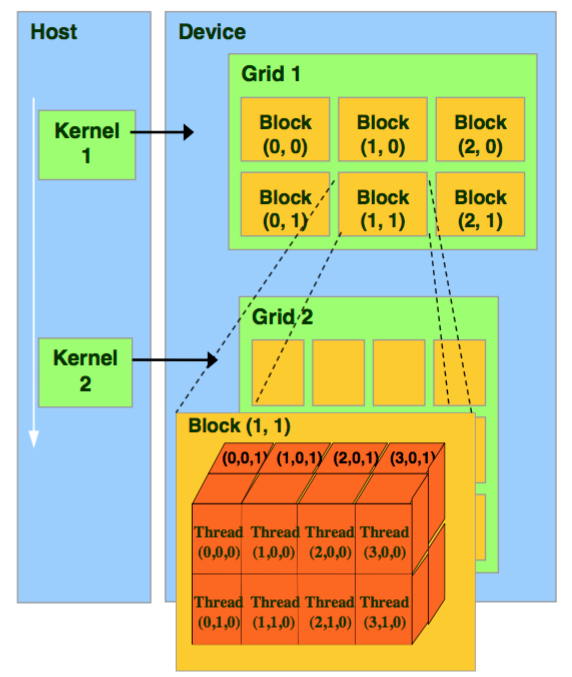
\includegraphics[width=0.4\textwidth]{images/grid_block_thread.png}
    \caption{Thread block abstraction model used in CUDA programming}
    \label{fig:gridblockthread}
\end{figure}

Each thread and block will have related positional indices that identify it within its parent container. This unique numerical identifier can be decomposed into N-dimensional coordinates (usually two or three dimensional) to perform arithmetic on a specific chunk of the data. Partitioning the data in this way allows for the vast parallelism as the programmer could submit an entire block or a small group of threads to the device for processing - there is a high level of fidelity granted to both data processing and transfer this way.

Before particulars of the CUDA technology are discussed, it's important to note that code that is written for CUDA must be exclusively compiled by the \texttt{nvcc} compiler provided in the CUDA Toolkit. General-purpose CPU code still needs to be compiled by the standard C compiler that is a part of the distribution you are developing for. This could present issues when trying to use several specialised compilers in tandem to provide a solution that utilises multiple technologies together.

\begin{itemize}
    \item Sync and parallelisation: thread cooperation, events.
    \item Streams
    \item Memory: Shared, Constant, Texture.
\end{itemize}

\subsubsection{Parallelisation and Synchronisation}

\subsubsection{Streams}

\subsubsection{Memory: Shared, Constant, Texture}



%%%%%%%%%%%%%%%%%%%%%%%%%%%%%%%%%%%%%%%%%%

\section{Design}
\label{sec:design}

Principally, the aim of this project is to establish, as a proof-of-concept, whether an existing code base can be meaningfully accelerated using CUDA technologies. A complete rewrite is not the goal as SNAP is a legacy project.

Establishing the efficacy of the proposed solution will be done against a best-case scenario model of parallel execution. Knowing this model is not attainable in practice for this project is acceptable (and not in scope). It will serve as a solid basis for future work should a complete refactor or related work be undertaken.

Following the conceptual, pure model, potential designs are remarked upon with their advantages and disadvantages highlighted, and supporting programs specified afterwards.


\subsection{Mathematical Model}
% TODO: Go over

In order to understand the amount of reasonable work the GPU could handle at once, as well as estimates for the amount of time and data movement needed for the optimal implementation, a mathematical model was developed to help visualise and describe the interactions between adjacent cells in the approximated algorithm that SNAP uses. The following assumptions were made when developing this model:

\begin{enumerate}

\item The algorithm defines the problem space as a three-dimensionally discretised grid of cells, each with their own values and interactions with their neighbouring adjacent cells. This forms the core of the SNAP algorithm (it itself approximating a continuous algorithm).

\item The problem space is cubic with side $ n $ for ease of modelling. A generalisation to a cuboidal space with dimensions $ (x, y, z) $ can be abstracted from the cubic model at a later time. A cubic model is conceptually and mathematically more intuitive to model.

\end{enumerate}

\begin{figure}[h!]
\centering
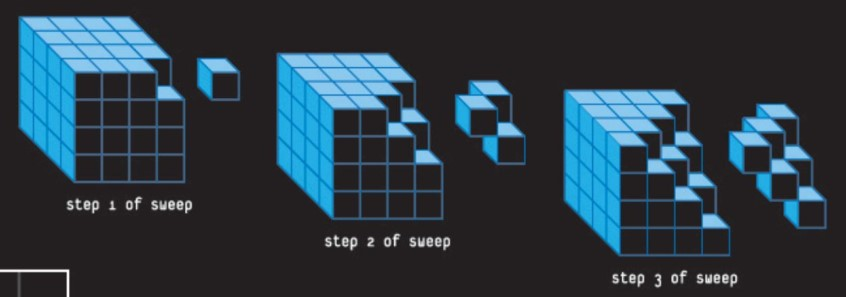
\includegraphics[width=0.45\textwidth]{images/Sweep.jpg}
\caption{Slices of a sweep of 3D grid}
\label{fig:3dsweepslice}
\end{figure}

Given these assumptions, we aim to derive the total number of communications between cells in the grid per iteration and how much work this equates to and how much can be parallelised at each stage.

There are $ 8 $ vertices of a cube so $ 8 $ octants to perform the sweep over. Each sweep is divided up into diagonal slices, shown in Figure \ref{fig:3dsweepslice}, of which there are $ (x + y + z) - 1 $ of them ($ 3n - 1 $ in this model). A key point to note is the dependency in each sweep of a slice on the slice before as the direction of the sweep is linear and calculations rely upon previous ones\footnote{As described in the documentation of the SNAP algorithm in their GitHub repository - \url{ https://github.com/lanl/SNAP/blob/master/docs/SNAP-overview-presentation-2015.pdf}}, and each combined sweep of all octants, after all results being collated, forms the basis of the next sweep.

The first $ n $ slices of the grid are comprised of the sum of the first $ n $ triangular numbers’ (i.e. $ 1, 3, 6, 10, 15\dots $)\footnote{Sequence A000217 in the ``On-line Encyclopedia of Integer Sequences'' (\url{https://oeis.org/A000217})}, worth of cells, with the final $ n $ slices having the same number also (just in reverse order). $ n - 2 $ slices exist between the 2 triangular-based pyramids formed from the previous step, allowing us to develop a function for the first $ m = n + \frac{n - 2}{2} $ slices, and mirror it to get the number of cells in any slice of the grid.

The number of cells in slice $ i $ of a cube of size $ n $ is thus given by the following formula:

\begin{equation}
cells(i) = \left\{
	\begin{array}{ll}
		tri(i) & \mbox{if } i \le n \\
		tri(i) - 3tri(i - n) & \mbox{if } i \le m \\
		cells(m - ((i - 1)\bmod m)) & \mbox{otherwise}
	\end{array}
\right.
\end{equation}

Where $ tri(i) $ represents the $i$th triangular number, $ 1 \le i \le 3n - 1 $. 

This means poor performance early on due to low numbers of cells per layer and the inter-slice dependency, but will ultimately scale well and to more graphics card given a large grid.

To work out data transfer, we need to figure out the amount of sends and receive actions are performed per slice. We can again work first out up to the first $ m $ slices, and take the mirror image for the rest of the slices, swapping the number of sends per slice for the receives of the mirror slice and vice versa. For the first $ n - 1 $ slices, each cell sends to 3 neighbouring adjacent cells in the next slice. When $ i \ge n $, we need to take into account the ``cut-off'' portions where some cells only send to 2 neighbours, hence:

\begin{equation}
sends(i) = \left\{
	\begin{array}{ll}
		tri(i) * 3 & \mbox{if } i < n \\
		(i\bmod(n - 1)) * 2 + \\
			(cells(i) - i\bmod(n - 1)) * 3 & \mbox{if } i \le m \\
		recvs(2n - i) & \mbox{otherwise}
	\end{array}
\right.
\end{equation}

The total number of receive actions is similar. The first cell has no neighbours to receive from, the second slice has only 1, the rest have three, then after the $n$th slice we need to consider where we only receive from 2 neighbours:

\begin{equation}
recvs(i) = \left\{
	\begin{array}{ll}
		0 & \mbox{if } i = 1 \\
		tri(i) & \mbox{if } i = 2 \\
		tri(i) * 3 & \mbox{if } i \le n \\
		(cells(i) - (2n - i)) * 3 & \mbox{if } i \le m \\
		sends(2n - i) \mbox{otherwise}
	\end{array}
\right.
\end{equation}

Both functions are defined in the domain $ 1 \le i \le 3n - 1 $.

If we let $ msg_s $ be the size of a message to send and $ msg_r $ the size of a message to receive from a neighbour (both in number of bytes), and knowing that the fastest data transfer rate of the PCI Express (PCIe) 2.0 bus connecting the graphics card and CPU together is 500MB/s\cite{PCIe}, we can calculate the time per slice to store data from the GPU as

\begin{equation}
time_s = \frac{sends(i) * msg_s}{5 \times 10^8}
\end{equation}

and to send data to it as

\begin{equation}
time_r = \frac{recvs(i) * msg_r}{5 \times 10^8}
\end{equation}

Aggregating these over all slices, alongside an assumed small, constant kernel function calculation time $ C $ over $ cells(i) $ cells in the slices, yields the best-case calculation time for the current approach. From here, we can interleave all 8 octants for calculation at once (of course managing the number of streaming multi-processors, which, after a point, we'd need to vastly scale hardware or queue work) to improve our throughput. $C$ ultimately depends on the type of graphics card being used.

\subsection{Ideation}

\begin{itemize}
    \item In-place replacement
    \item Loop flattening
\end{itemize}

\subsection{Test Harness}

In order to accelerate the process of testing, analysis, and comparison of data and timings yielded from the runs of the two separate SNAP variants, a decision was made to create a test harness program that will automate the process of running and collecting results.

Automation with regards to testing is key to repeatability, reproducibility, the speed at which results can be obtained, and general accuracy of the results. Hence, for testing of both programs to be effective, the test harness program must meet certain criteria in a holistic process to ensure the project is a success. The overall aims of the program are: to act as a wrapper to run both versions of the program with; to provide high-precision timing of executions; to handle any errors thrown; and to output, compare, and save the results of executions for analysis and reporting.

Firstly, the program should act as a wrapper to the execution of both programs. Manual execution of the programs is slow, can be inaccurate, parameters can be missed accidentally, and executing a sequential string of commands, each varying a little (e.g. only changing the input and output destinations) is tedious. Programmatic control will expedite the testing process and provide extra flexibility should the testing process need to be enhanced or altered in the future.

Further to this is, crucially, accurately timing the execution of both programs. It would be an ineffective solution to the problem if the GPU-accelerated version of SNAP would be routinely slower than the original. Specifically, timing both the entire execution of the program and the internal algorithm/function we're seeking to modify would give an overall impression of the efficacy of the solution. For example, if the algorithm's execution time has decreased but the overall program's execution time has increased due to knock-on factors as a result, then the solution would need further work.

Advanced control could not be achieved if the harness were not able to capture output and errors of the underlying programs that it was calling. It's important to know when errors are found as it might be necessary to halt the problem and report it or continue on regardless depending on what happened - the solution needs to provide this support and subsequently handle it. To this end, obtained the output of both of the programs is a required detail to analyse problems, but most importantly, to compare the final numerical results of the execution on identical inputs to ensure that the results are the same. Inconsistent results mean an improper, incorrect solution. This comparison and analytical process needs to also be in part to mostly automated to save users from wasting time doing it manually and potentially not spotting a discrepancy or difference.

A program that meets these central requirements will act as an effective and useful testing tool for assessing if the end solution meets the objectives of this project.


%%%%%%%%%%%%%%%%%%%%%%%%%%%%%%%%%%%%%%%%%%

\section{Implementation}
\label{sec:implementation}

An experimental alteration to an existing code base can often be wrought with challenges. Therefore, a solution to this problem that meets all the objectives outlined earlier must satisfy the following criteria:

\begin{itemize}
    \item \textbf{Accuracy} - Simply put: if the results of the program after the modification do not align with the results of the unmodified program, then the solution is not satisfactory and is thus incorrect. Care and constant ratification must be performed often to ensure this trait is maintained as development occurs.
    \item \textbf{Speed} - A solution that is not better than or comparable to the existing program's performance is worse in practice. In the worst case, the program should be at least as fast.
    \item \textbf{Simplicity} - A solution that is conceptually harder than the existing code is not only not as maintainable but increases the fragility of the algorithm. Code that is improved \textit{and} intuitive can lead to further improvements down the line such as performance gains, reduction of necessary code, or easier parallelisation.
\end{itemize}

Accuracy and speed are easily assessed using simple comparative automations and time-keeping. These were the key motivators for introducing a test harness program into the development and testing cycle (see Subsection \ref{subsec:imp_testharness} for development details). Simplicity is a more subjective metric for evaluating a software-based project. A best-attempt at an objective review of the implementation will be featured in the conclusion (Section \ref{sec:conclusion}). However, personal preference and opinion will always factor into such a review, so the reader can also review the code base provided to make up their own mind.

Development was undertaken iteratively after installation of all of the necessary prerequisites to start programming. The basic cycle mimics aspects of the Agile development cycle\footnote{\url{https://www.agilealliance.org/agile101/}} and other traditional development cycles:

\begin{enumerate}
    \item Partition the current problem into a list of remaining sub-problems.
    \item Write code to solve the current sub-problem.
    \item Test the code.
    \begin{enumerate}
        \item If it works, move forward to step 1.
        \item Else, go back to step 2.
    \end{enumerate}
\end{enumerate}

This project diverges from this slightly in that during the second stage code was written for both the CUDA-based alteration and the test harness. As one was developed, the other was developed and tweaked further. Both were kept in step to ensure accuracy and speed. Implementation details of component of the project follow.


\subsection{Prerequisites}
\label{subsec:imp_prerequisites}

To begin development, in addition to the installation of the necessary Ubuntu packages for C/C++ compilation and python development, it's necessary to install binaries associated with the CUDA development kit and runtime.

A proprietary device driver for Nvidia graphics cards on Ubuntu is required for CUDA code to run on the device. This is provided as part of the ``CUDA Toolkit'' that is freely available to all developers from Nvidia's Developer portal \url{https://developer.nvidia.com/cuda-downloads}. Installation is a matter of following the steps in the installer. It was important to note that the driver provided with the installer is the one guaranteed to work with the CUDA Toolkit, as opposed to the ones provided as part of the operating system vendor's software package ecosystem. Modification of the \texttt{PATH} and \texttt{LD\_LIBRARY\_PATH} to reference the \texttt{/usr/local/cuda-10.1/*}\footnote{The latest CUDA Toolkit version at time of development.} folders sets up the running environment properly and, with careful compilation, now allows for compilation and execution of CUDA code via the \texttt{nvcc} compiler.

One last prerequisite is to have the Intel MPI libraries installed an operational on the development machine also. This is covered in Subsubsection \ref{subsubsec:inv_compilation}.


\subsection{Test Harness}
\label{subsec:imp_testharness}
% TODO: Finish

Developed in conjunction with the modified SNAP application (Subsection \ref{subsec:imp_mod_snap}), the test harness program is a versatile complementary program that aims to help achieve the objectives of the project by providing the following features:

\begin{itemize}
    \item Acts as a wrapper to both CPU and GPU-augmented versions of the SNAP programs.
    \item Precisely times their execution.
    \item Compares outputs of the programs to gauge consistency.
\end{itemize}

For this supplementary program, Python version 3.7+ will be the main implementation language. The core libraries of Python, in conjunction with its ease of development and portability will allow the program to be developed rapidly and be more intuitive. Version 3.7.3 is used explicitly due to its modernity (it was the latest available distribution at the time of writing) and this script's reliance on the \texttt{time.time\_ns()} function (the use of which is described later).

Three of the main APIs utilised in the program that meet most of the needs of the above requires are the \texttt{os}, \texttt{subprocess}, and \texttt{time} libraries found in Python's standard set of core libraries. These libraries provide tight, low-level, flexible interfaces for working with the host operating system in addition to providing high-precision timing facilities for program comparison and profiling. Further advantages are discussed as the implementation details of each point are outlined in turn.

The primary goal of the test harness program is to act as a wrapper to execute either one of the SNAP programs. This control allows for a fine-level of timing and parameter control that isn't guaranteed with manual execution. Python's \texttt{subprocess} library can interoperate with Ubuntu and execute shell commands specified by strings in the script and have them execute within a subprocess. Not only does this provide exact start and end times of when the underlying subprocess is forked and joined back into the main executing process, but the library provides an extensive API to handle and report errors, output, and stream input for a variety of sources, amongst other features. Specifically, \texttt{subprocess.call([\dots])} is liberally utilised as it takes in an array of parameters (the head of which being the program binary name) and executes it as if it were a shell command. Programmatically inserting input parameters, the path of the SNAP binary - chosen by an argument passed into the \texttt{test.py} script itself - to execute, as well as any additional information and arguments for manipulating the execution or profiling characteristics (see Subsubsection \ref{subsubsec:testapi} for further details). If it is ever the case that written algorithms in the script could be deferred to an existing piece of software or bash script (e.g. \texttt{diff} or \texttt{cmp}) then this could also be used to refactor the program to utilise those instead.

The \texttt{os} library handles difference between operating systems types to make the program as OS-agnostic as possible. Details such as file path separators, reading, and writing are handled through a common API. This allows for easy reading of an input or output file into the program for line-by-line parsing by several other routines and libraries used for the other stages and parts of the script. \texttt{os.remove} is used to delete the extraneous \texttt{gmon.out} files produced by profiling, while \texttt{os.path.join} is used to link scripted parts of paths together to find the output directory and particular files within it for averaging of execution times and comparison of the contents of the files - alongside the \texttt{open(\dots)} function from standard Python.

High-precision timing is provided by the \texttt{time} library: specifically, the \texttt{time.time\_ns()} function. This function was introduced in Python 3.7 when nanoseconds resolution was introduced to the \texttt{time} library\footnote{\url{https://docs.python.org/3.7/whatsnew/3.7.html#pep-564-add-new-time-functions-with-nanosecond-resolution}}. Precision and accuracy is key when doing time-based profiling specifically, hence the require for the nanosecond time resolution. \texttt{time} previously only had the \texttt{time.time()} function which only returned the number of seconds since a certain date, i.e. Unix epoch time, and this was certainly not appropriate. 

Detailed breakdowns via the use of \texttt{MPI\_Wtime()} to time the start and end times of the \texttt{dim3\_sweep} function and its parent subroutines in the call stack were experimented with. The cost of the intricate implementation of summing all the values from all of the MPI processes outweighed the benefit of the insight it would provide so this was not included in the final build. Use of \texttt{gprof} and other profilers provide similar functionality already.

% TODO
% Diffing outputs
% Cleaning timestamps, separating time blocks

\subsubsection{\texttt{test.py} API}
\label{subsubsec:testapi}

The test harness assumes the form of a program operated solely via the command-line. As such, there is a small set of commands and arguments associated with the various functionalities implemented and described in the design. A reference follows, all of which can be accessed via a terminal by issuing the command \texttt{python test.py -h}.

\begin{itemize}
    \item \textbf{setup}: Establishes the executing environment if not already configured.
    \item \textbf{clean}: Cleans any superfluous or unnecessary files from profiling or previous runs that are otherwise cluttering up the working directory.
    \item \textbf{run}: Executes one of the SNAP binaries in the project using the following arguments:
    \begin{itemize}
        \item \textbf{--cpu}: Makes the program choose the original binary file of the SNAP program. Must define either this flag or \textbf{--gpu}.
        \item \textbf{--gpu}: Makes the program choose the modified, GPU-accelerated binary file of the SNAP program. Must define either this flag or \textbf{--cpu}.
        \item \textbf{-n, --np}: Number of MPI processes to run with.
        \item \textbf{-i, --fi}: Path to the input file to test the program with. 
        \item \textbf{-o, --fo}: Path to write the output of the program to.
    \end{itemize}
    \item \textbf{analyse}: Performs a set of comparative analyses on the output of both CPU and GPU-enabled programs and produces a report and several files detailing the differences between the two sets of results.
\end{itemize}

The following global flags are also available for any command:

\begin{itemize}
    \item \textbf{-v, --verbose}: Increase the amount of output of the program for diagnostics.
\end{itemize}


\subsection{Modified SNAP Application}
\label{subsec:imp_mod_snap}

Developing the GPU-accelerations for SNAP first involved understanding how to integrate the CUDA algorithms into the existing MPI-based C implementation.

It was required to get both the \texttt{nvcc} and \texttt{mpiicc} to co-operate with one another, first and foremost.

Secondly, in terms of the process of development, was to attain an understanding of how best to integrate CUDA and MPI code together. An issue presented immediately is that of both the specialised compilers splitting the compilation process into stages. Each compiler will compile separately the specialised parts of the code that the standard C/C++ compiler does not know how to handle, whilst, either at the same time or after the first stage, it will call the standard, underlying compile to compile the rest of the source files. Afterwards, the specialised compile will link both compile non-standard and standard object files together into one executable binary file. Having both compilers do this process means that specialised MPI and CUDA code may not be able to easily co-exist in the same source code files without separation or careful orchestration of the build process.


\subsubsection{\texttt{nvcc} and \texttt{mpiicc}}
% TODO: 


\subsubsection{Externalised CUDA Algorithms}
% TODO:

%%%%%%%%%%%%%%%%%%%%%%%%%%%%%%%%%%%%%%%%%%

\section{Testing}
\label{sec:testing}
% TODO:
% Test plan
% Local Testing + Results
% Cluster Testing + Results
% Analysis

Verification of the modified software will take place in two stages on different sized platforms, as outlined in subsubsections \ref{subsubsec:projmgmt_localtesting} (Local Development Platform) and \ref{subsubsec:clusters} (Computing Clusters) so see if the code scales. The primary objective is to attempt to observe a time-decrease over every problem size in the best case scenario. Other objectives are:

\begin{itemize}
    \item Ensuring the modified solution produces the same results as the original version is all circumstances.
    \item A subsequent secondary performance increase is observed in multi-GPU environments. This is supplementary and not required, as CUDA has particular technologies associated with distributed work across multiple devices.   
\end{itemize}

There are a couple of main variables that would immediately effect the performance of both programs: the number of CPU threads, the amount of MPI processes, and the block and thread configurations of all CUDA-based kernel function calls. Several variations of these will be incorporated into the testing as they will show trends in parallelism that might not otherwise be observed if just a few fixed values are used. For instance, it may be the case that the algorithm doesn't scale well to higher numbers of processes or threads.

\subsection{Test Plan}
\label{subsec:testplan}

To meet these objectives, the following test plan is laid out. Cluster-based testing may be omitted depending upon the results obtained during local testing - it may be the case that there is no apparent performance increase.

Starting with local testing:
\begin{figure}[!h]
    \centering
    \begin{tabular}{|l|l|}
        \hline
        Value 1 & Value 2 \\
        \hline
        1 & 2 \\
        \hline
    \end{tabular}
    \label{table:localtestplan}
\end{figure}

Once, and only if, all of the testing has passed up until this point, we can proceed with cluster-based testing:

\begin{figure}[!h]
    \centering
    \begin{tabular}{|l|l|}
        \hline
        Value 1 & Value 2 \\
        \hline
        1 & 2 \\
        \hline
    \end{tabular}
    \label{table:clustertestplan}
\end{figure}


\subsection{Local Testing Results}
\label{subsec:testing_local}

\subsection{Cluster Testing Results}
\label{subsec:testing_cluster}

\subsection{Results}
\label{subsec:results}


%%%%%%%%%%%%%%%%%%%%%%%%%%%%%%%%%%%%%%%%%%

\section{Conclusion}
\label{sec:conclusion}

\subsection{Limitations}
\label{subsec:limitations}

\begin{itemize}
    \item Very proprietary code base
\end{itemize}

\subsection{Improvements}

Over the course of the project, several issues or development quirks came to light in almost every aspect of the pipeline. Several key improvements that could be made to the project are presented below that could rectify these should subsequent or related projects take on a similar endeavour to the one presented in this report:

\begin{itemize}
    \item \textbf{Texture memory}: One core feature in the CUDA library that wasn't explored due to learning the legacy code base, pursuing alternative designs, and other time constraints, is texture memory and the potential solution and performance benefits it could bring. Texture memory is specialised, cached memory that improves the memory bandwidth of a running parallel application by exploiting the spatial locality of the data in question, as in the following figure:
    
        \begin{figure}[H]
            \centering
            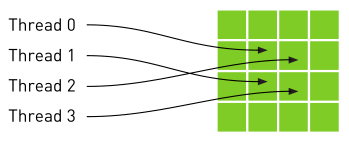
\includegraphics[width=0.4\textwidth]{images/TextureMemory.png}
            \caption{Thread-based access of texture memory}
            \label{fig:texmem}
        \end{figure}
    
    For restricted transport-sweep problems over two dimensions, texture memory for the implementation of the grid would greatly speed up reads from memory. Each thread can operate a different directional sweep across the same cached texture, synchronise all of the threads, and aggregate the results back before transferring data back to main memory and the CPU. 

    This approach has promise and would be ideal to pursue further for problems like SNAP.

    \item \textbf{Containerisation}: An issue that appeared time and again during the initial investigation stages was the lack of other projects that had tied together MPI and CUDA as this project was seeking to do. Whilst not unusual for new and novel work, the lack of supporting documentation for this use-case proved to be a hinderance to time and slowed parts of the project down. A key piece of future work for this project in the future could be the establishment of a Docker container (a software housing that guarantees consistency of execution no matter what hardware it is run on) to hold binaries and settings for future release and other researchers to use the technologies together, alongside supporting documentation detailing lessons learned during the course of development.

    \item \textbf{Standardised input data format}: Modernising and documenting the input data structure would help to vastly improve the fidelity and flexibility of the program by allowing faster and more intuitive changes to be made without prior knowledge. As it stands, the input format is very proprietary and analysis of the code, particularly \texttt{input.c}, is needed in order to interpret the variables and what they mean in context.
    
    Utilising a modern, global data standard such as JSON or XML over a whitespace dependent ordering would increase the usefulness of input files used for testing. Not only are there high-performance, fast, compact parsing libraries available for these formats but they're also intrinsically easier to document and modify.

    \item \dots

\end{itemize}

%%%%%%%%%%%%%%%%%%%%%%%%%%%%%%%%%%%%%%%%%%

\bibliographystyle{ieeetr}
\bibliography{dissertation}

\end{document}